% !TEX encoding = UTF-8 Unicode
\documentclass{article}
\usepackage{geometry} % 設定邊界
\geometry{
  top=2in,
  inner=1in,
  outer=1in,
  bottom=1in,
  headheight=3ex,
  headsep=2ex
}

\usepackage{fontspec}   %加這個就可以設定字體
\usepackage{xeCJK}       %讓中英文字體分開設置
\setCJKmainfont{BiauKai} %設定中文為系統上的字型,而英文不去更動,使用原TeX字型
\setmainfont{Times} % 設定英文字型
\XeTeXlinebreaklocale "zh"             %這兩行一定要加,中文才能自動換行
\XeTeXlinebreakskip = 0pt plus 1pt     %這兩行一定要加,中文才能自動換行

\usepackage{titling}
\setlength{\droptitle}{-12em} % 將標題移動至頁面的上面


\title{第五章: 物體辨識與ROS Package應用}

\author{蘇詠善}
\date{} %不要日期

\begin{document}
\maketitle

本章節將帶領學員活用Open Source Computer Vision Library (OpenCV)實踐物體辨識,並把OpenCV與ROS Package結合在一起,讓車子執行123木頭人。此章節一共分為三大部分:物體辨識、如何創造ROS Package、123木頭人專題教學。在學習完此章節後你將能熟悉OpenCV、Python、Jupyter-Notebook、ROS Package。
\section{物體偵測}
課程目標:學生能熟悉如何使用OpenCV,並在程式平台Jupyter-Notebook上實踐。
\\需先備知識與需先安裝好的資料庫:
\\程式平台Jupyter-Notebook
\\開源電腦視覺函式庫OpenCV
\\開源程式Python

\subsection{基本介紹:}
Jupyter-Notebook為一個十分便於編譯python的平台,它不僅有圖形介面且也能即時的顯現執行程式的結果,因此為了讓學員們能熟悉運用OpenCV,本章將以Juputer-Notebook為平台一步一步帶領大家熟悉OpenCV,並運用此平台實踐物體偵測的演算法。
\\\\步驟一、開啟Jupyter-Notebook
\\duckietown \$ cd ~/duckietown/tutorials/python/
\\進入到範例程式檔所處的資料夾
\\duckietown \$ jupyter-notebook 01-tutorial-object-detector.ipynb
\\開啟範例程式
\\\\步驟二、讀取所有所需的函式庫
\\由於接下來要寫的程式會運用到大量的函式庫,此區的程式將會讀取數學函式庫(numpy)、科學計算函式庫(scipy)、開源電腦視覺函式庫(cv2)、時間函式庫(time)、繪圖函式庫(pyplot)
\
\begin{figure}[htp]
    \begin{center}
        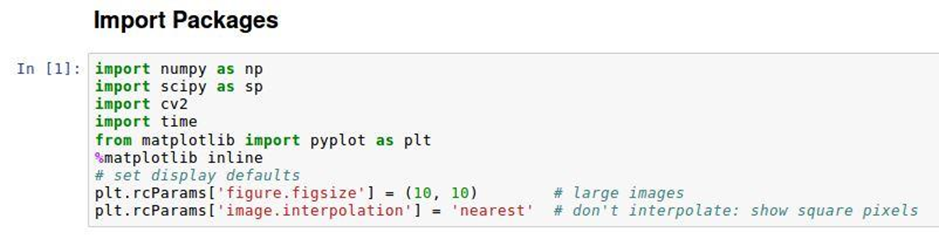
\includegraphics[width=400pt]{pic/5_1_1.png}
    \end{center}
\end{figure}
\\
步驟三、執行範例程式
\\邊緣偵測
\\在物件偵測中,邊緣偵測是一個相當重要的工具,因為它能將圖形的細節給表現出來,因此這部分所示範的是將一張圖片讀取後,進行坎尼邊緣偵測(Canny edge detection),並將結果與原圖視覺化以進行比較。
\
\begin{figure}[htp]
    \begin{center}
        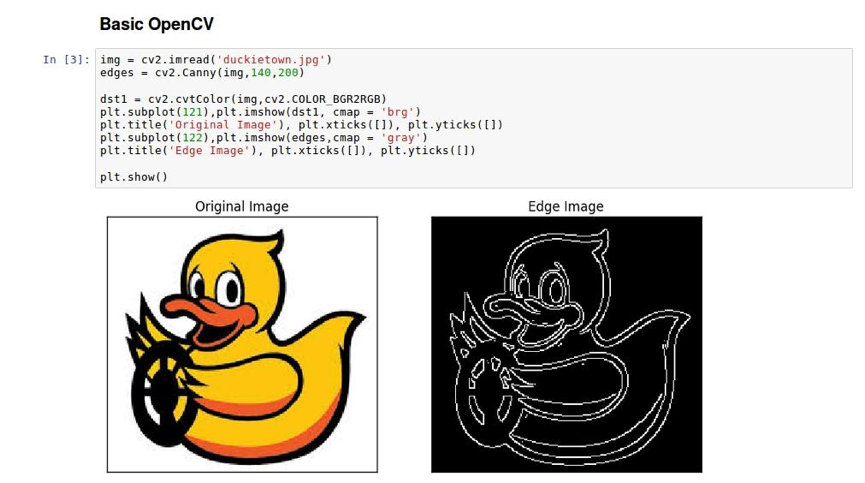
\includegraphics[width=400pt]{pic/5_1_2.png}
    \end{center}
\end{figure}
\\
\\\\藉由圓形圖案來辨識車子
\\本小節我們會在車子背後貼圓形圖案,並藉由斑點辨識(blob detection)來辨識圓形圖案。程式將會先將圖片讀取進來後,再宣告一些基本變數,最後使用OpenCV函式庫所提供的斑點辨識函式來辨識圓形圖案,並將辨識到的圓形圖案視覺化。
\
\begin{figure}[htp]
    \begin{center}
        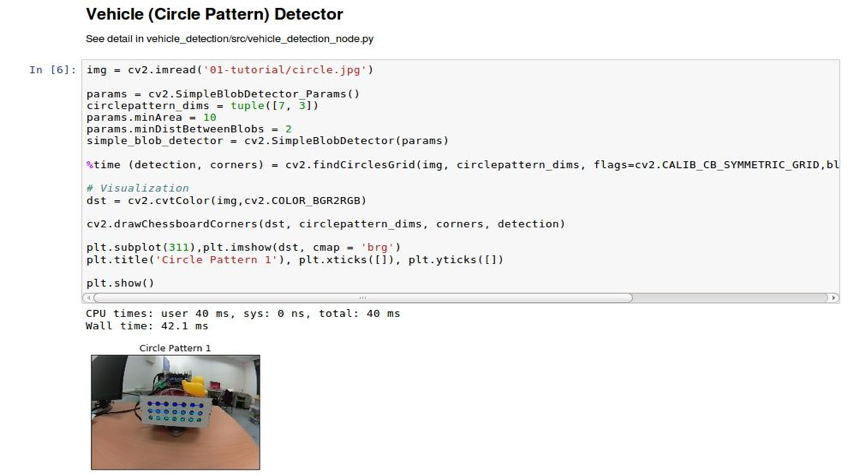
\includegraphics[width=330pt]{pic/5_1_3.png}
    \end{center}
\end{figure}
\\
函式代表意義 : 
\\cv2.simpleBlobDetector\_Params()	: 設定斑點辨識 (blob detector)的參數  
\\tuple()						: 設定要找到的圓圈的行與列.
\\params.minArea() 				: 設定斑點辨識要尋找圈圈涵蓋的最小區域
\\params.minDistBetweenBlobs 	: 設定斑點辨識要尋找圈圈之間的最短距離
\\cv2.findCirclesGrid 				: 找到圓圈
\\cv2.drawChessboardCorners 		: 在偵測到的圈圈之間畫線
\\\\臉部偵測
\\本小節我們使用了OpenCV裡的串接式決策分類器(Cascade Classifier),使用現成的訓練模型來辨識人臉。因此在這部分的程式,會先讀取圖片及訓練模型,在設定一些基本參數後,進行辨識。最後再將人臉框出來,並視覺化。
\
\begin{figure}[htp]
    \begin{center}
        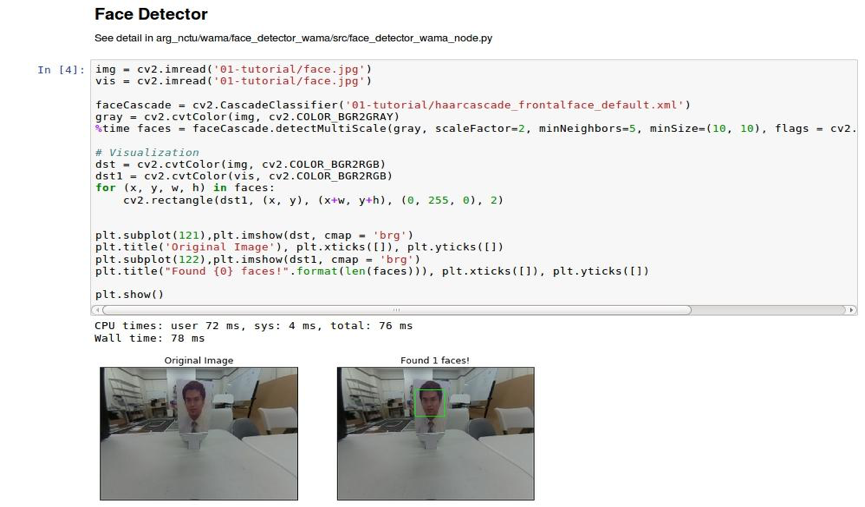
\includegraphics[width=400pt]{pic/5_1_4.png}
    \end{center}
\end{figure}
\\
函式代表意義 : 
\\cv2.CascadeClassifier()	: 讀取串接式決策分類器(cascade classifier)
\\detectMultiscale()		: 設定串接式決策分類器(cascade classifier)參數
\\scaleFactor			: 設定要將圖片放大幾倍
\\minNeighbors			: 指定每個候選矩陣至少包含的鄰近元素個數
\\minSize / maxSize	 	: 設定偵測物體在圖片中尺寸的極值
\\flags				: reference/tag refer to the old feature
\\cv2.rectangle()		: 畫出一個矩形
\\\\物體辨識(以鴨子為例)
\\這一部分會分解成三個小部分,第一部分為運用HSV色彩辨識偵測鴨子。第二部分則是寫下運用輪廓來辨識鴨子的演算法,最後一部分則是使用第二部分的演算法來偵測鴨子。
\\第一部分先讀取圖片後,將圖片轉成HSV色彩空間,再藉由HSV色彩辨識的方式將鴨子身體的顏色(黃色)給濾出來,最後進行視覺化。
\begin{figure}[htp]
    \begin{center}
        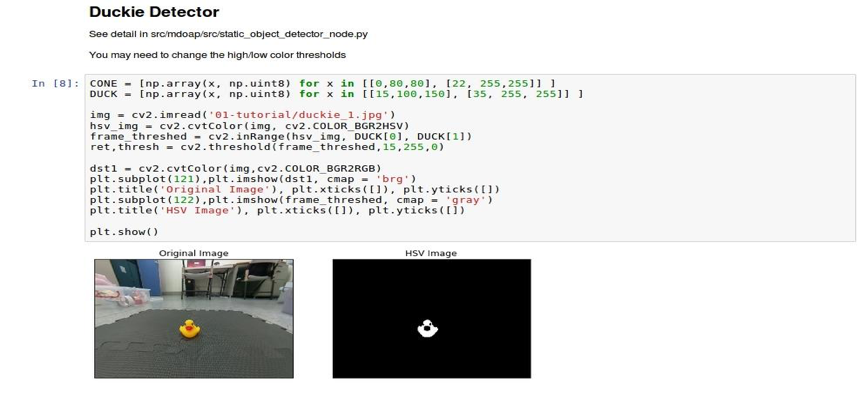
\includegraphics[width=400pt]{pic/5_1_5.png}
    \end{center}
\end{figure}
\\
函式代表意義 : 
\\np.array			: 建立新的陣列
\\cv2.inRange()		: 設定範圍
\\cv2.threshold()		: 設定門檻值
\\\\第二部分則是鴨子偵測演算法的函式,待會會被使用到。
\\函式代表意義 : 
\\cv2.findcontours()			: 找到二元影像的輪廓
\\cv2.RETR\_CCOMP()		: 建立兩個等级的輪廓,上面的一層為邊界,里面的一層為内孔的邊界信息。
\\cv2.CHAIN\_APPROX\_SIMPLE()	: 壓縮水平、垂直、對角方向的元素,只保留該方向的終點座標
\\cv2.contourArea()			: 輪廓面積
\\cv2.boundingRect()			: 計算邊界矩形
\\cv2.arcLength()			: 計算輪廓周長
\\cv2.drawContours()			: 使用得到的點劃出輪廓與形狀
\\\\最後一部分將用前一部分所寫好的函式來偵測鴨子的輪廓,如果偵測到的輪廓有吻合鴨子的輪廓,程式將會將鴨子偵測出來,且框出它,並視覺化。
\begin{figure}[htp]
    \begin{center}
        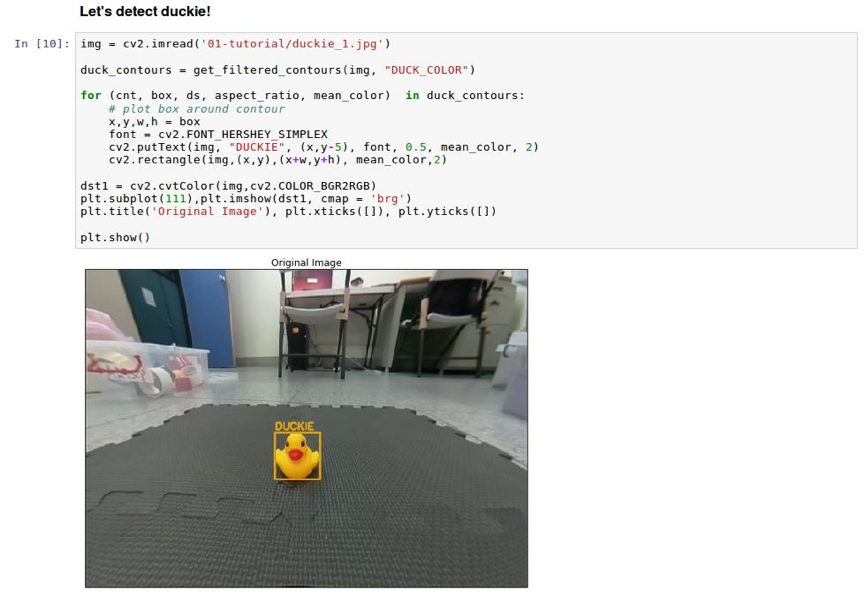
\includegraphics[width=300pt]{pic/5_1_6.png}
    \end{center}
\end{figure}
\\
\\\\\\\\\\\\\\\\\\\\\\\\\\\\\\\\\\\\最大穩定極值區域(Maximally Stable Extremal Regions)
\\此部分為示範運用最大穩定極值區域的概念來將圖片切割成許多小塊,每一個小塊都是一個輪廓。程式中,會先讀取圖片,並將圖片轉成灰階圖,接著使用OpenCV的MSER函式來將圖片切成許多小塊的輪廓並視覺化。
\begin{figure}[htp]
    \begin{center}
        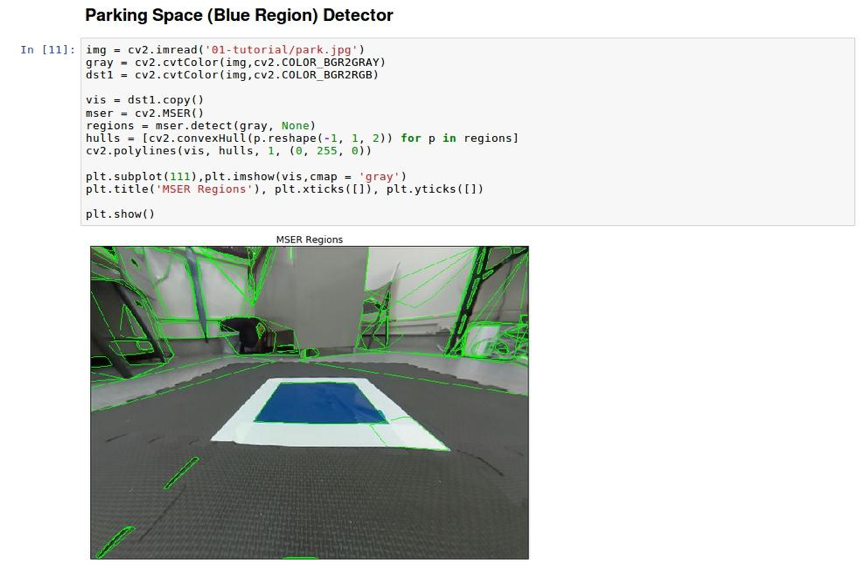
\includegraphics[width=300pt]{pic/5_1_7.png}
    \end{center}
\end{figure}
\\
函式代表意義 : 
cv2.MSER()			:回傳所有圖片中偵測到的點
cv2.convexHull()		:將那些點連接起來

\subsection{牛刀小試:}
臉部偵測器乃本章最為複雜的演算法之一,請你嘗試善用本章教過的串接式決策分類器來對以下兩張圖片進行臉部辨識,將所有的臉部都偵測出來。
\\(提示:針對不同的圖片,參數的調整也都會不一樣。)

\newpage
\section{創造一個ROS package (Python)}
課程目標:學生能熟悉如何創造ROS package
\\需先備知識與需先安裝好的資料庫:
\\需先安裝好機器人作業系統(ROS)

\subsection{ROS基本介紹:}
ROS是現今最流行的機器人作業系統,國際名校如史丹佛大學、麻省理工學院皆廣泛使用這套系統。我們已於前幾章介紹過ROS的概念,在本小節我們將進行實作。我們會先學習創建一個ROS package需要打那些指令、引進不同的函式庫需要去改那些檔案。最後去學習將事先已寫好的launch檔進行修改,然後跑起來。我們一共會分為六個步驟:第一步驟會先把主要的package先創立出來。第二步驟會創造出一個launch檔,目的是去呼叫第三步驟會去創立的package中的launch,這個方式在往後會大量應用。第三、四、五步驟則是創立一個新的package及launch檔,並且會實作如何修改”CMakeLists.txt”與”package.xml”去連結函式庫,第六步驟是執行剛剛寫好的launch檔,並使用ROS的圖形化模擬環境RVIZ去將傳輸的訊息視覺化。
\subsection{ROS實驗步驟:}
步驟零、初始化 ROS環境與 ROS Master
\\此步驟是為了設定好ROS的環境,我們將ROS的環境架在”duckietown”這個資料夾底下,這個資料夾裡有兩個bash檔” environment.sh”和” set\_ros\_master.sh”,在使用ROS前我們必須先執行過這兩個bash檔,才能把ROS基本環境設定好,接著才能做之後創建ROS package的動作。
\\laptop \$ssh ubuntu@duckiebot.local
\\(指令解釋:用筆電連線到Pi上,進行遠端控制)
\\duckiebot \$ cd ~/duckietown
\\duckiebot \$ source environment.sh
\\(指令解釋:執行bash檔”environment.sh”)
\\duckiebot \$ source set\_ros\_master.sh [duckiebot]
\\(指令解釋:執行bash檔” set\_ros\_master.sh”)
\\\\步驟一、創造你的Ros package 
\\此步驟的目的是要創建一個完整的ROS package,因此我們使用到catkin\_create\_pkg”這個指令,它可以幫我們自動把package建好,且還會幫我們自動加入兩個檔案(“CMakeLists.txt”與” package.xml”),這兩個檔案定義了我們的程式可以使用哪些函式庫,因此十分重要。未來若想連結其他函式庫,也需去更改這兩個檔案。
\\duckiebot \$ cd ~/duckietown/catkin\_ws/src/summerschool2017\_nctu/
\\duckiebot \$ mkdir [duckiebot]
\\(指令解釋:創建新目錄”duckiebot”,創完後輸入指令”ls”,你會看到一個資料夾  (以duckiebot的名字來命名,那是你剛才創的)
\begin{figure}[htp]
    \begin{center}
        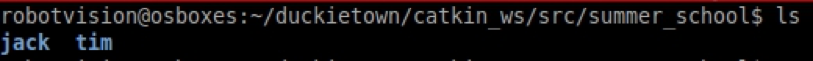
\includegraphics[width=400pt]{pic/5_2_1.png}
    \end{center}
\end{figure}
\\
duckiebot \$ cd ~/duckietown/catkin\_ws/src/summerschool2017\_nctu/[duckiebot]
\\duckiebot \$ catkin\_create\_pkg duckietown\_[duckiebot]
\\(指令解釋:創造ROS package “duckiebot”)
\\duckiebot \$ cd duckietown\_[duckiebot]
\begin{figure}[htp]
    \begin{center}
        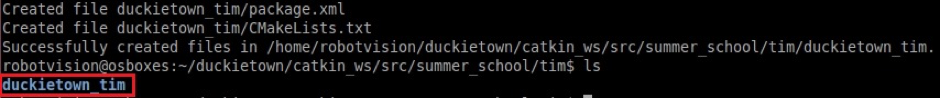
\includegraphics[width=400pt]{pic/5_2_2.png}
    \end{center}
\end{figure}
\\
步驟二、在”duckietown\_[duckiebot]”這個目錄底下創造名為launch的資料夾
\\前幾章已說明過launch對ROS的重要性與概念,因此為了建立launch檔,我們習慣先建立一個名為”launch”的資料夾,在這資料夾底下再去建立launch檔,因此在此步驟中便是教大家先建立資料夾,再去複製我們的範例launch檔到我們剛剛建立的資料夾底下。最後簡單修改範例launch檔後便完成。
\\duckiebot \$ mkdir launch
\\duckiebot \$ cd launch
\\duckiebot \$ cp ~/duckietown/catkin\_ws/src/spring2016\_nctu/wama/duckietown\_wama/launch/ros\_cv\_example\_wama.launch ros\_cv\_example\_[duckiebot].launch 
(指令解釋:將事先已寫好的範例程式複製到此資料夾底下,複製好後輸入指令”ls”,你會看到以下檔案  (ros\_cv\_example\_[duckiebit].launch)
\begin{figure}[htp]
    \begin{center}
        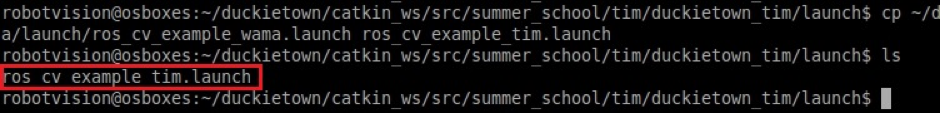
\includegraphics[width=400pt]{pic/5_2_3.png}
    \end{center}
\end{figure}
\\
duckiebot \$ vim ros\_cv\_example\_[duckiebot].launch
\\Modify the following: duckiebot=your duckiebot name
\\ <!-- ros\_cv\_example\_duckiebot-->
\\     <remap from="ros\_cv\_example\_duckiebot\_node/image" to="camera\_node/image/compressed"/>
\\     <include file="\$(find ros\_cv\_example\_duckiebot)/launch/ros\_cv\_example\_duckiebot\_node.launch">
\\(指令解釋:打開launch檔後需要按照以上方式將所有”duckiebot”改寫成你鴨子車的名字。)
\\\\步驟三、創造一個名為ros\_cv\_example\_[duckiebot]的ros package
\\在此步驟中,我們會再創立一個新的ROS package,在這個package裡,我們會先實作修改”CMakeLists.txt”與”package.xml”,將所有的資料庫都鏈結起來。
\\duckiebot \$ cd ~/duckietown/catkin\_ws/src/summerschool2017\_nctu/[duckiebot]
\\duckiebot \$ catkin\_create\_pkg ros\_cv\_example\_duckiebot 
\\duckietown\_msgs  geometry\_msgs roscpp rospy std\_msgs sensor\_msgs cv\_bridge
(指令解釋:創造ROS package “ros\_cv\_example\_duckiebot”,且加入一些需要用到的函式庫,輸入以上指令後你會看到以下結果)
\begin{figure}[htp]
    \begin{center}
        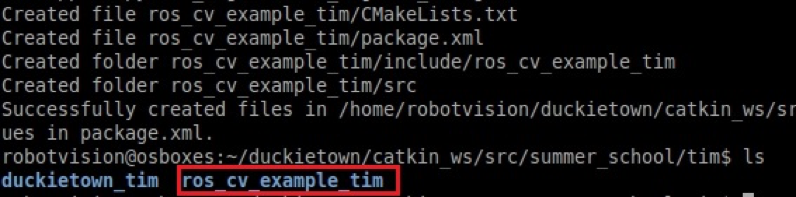
\includegraphics[width=400pt]{pic/5_2_4.png}
    \end{center}
\end{figure}
\\
(附註:加入的函式庫”duckietown\_msgs”、” geometry\_msgs”、”std\_msgs”、”sensor\_msgs”是ROS常用到傳遞訊息的ROS message的函式庫,而”roscpp”、” rospy”、” cv\_bridge”則是ROS與OpenCV的函式庫)
\\\\duckiebot \$ cd ros\_cv\_example\_duckiebot/
\\duckiebot \$ vim package.xml
(指令解釋:打開檔案後你會看到程式(如下),裡面有許多函式庫作為我們之後寫的程式的函式庫dependency)
\begin{figure}[htp]
    \begin{center}
        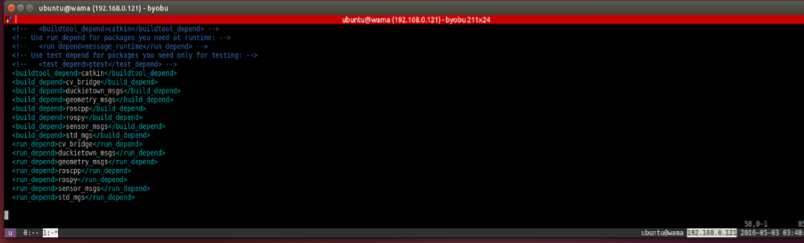
\includegraphics[width=400pt]{pic/5_2_5.png}
    \end{center}
\end{figure}
\\
duckiebot \$ vim CMakeLists.txt 
(指令解釋:打開檔案後你會看到程式(如下),請加入這一行“find\_package(OpenCV REQUIRED)”與加入這一行\${OpenCV\_INCLUDE\_DIRS}”如以下幾張圖的方式,目的是為了去找到函式庫OpenCV,如此之後去使用此函式庫才沒有問題。)
\begin{figure}[htp]
    \begin{center}
        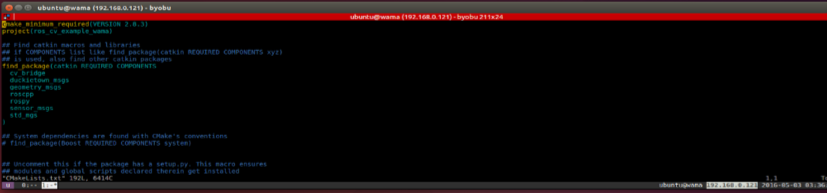
\includegraphics[width=400pt]{pic/5_2_6.png}
        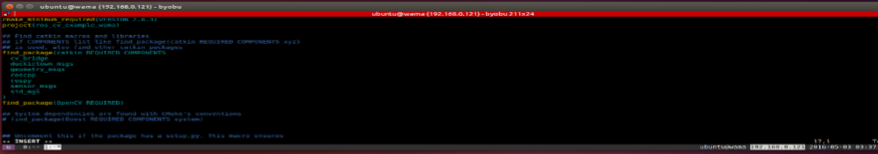
\includegraphics[width=400pt]{pic/5_2_7.png}
        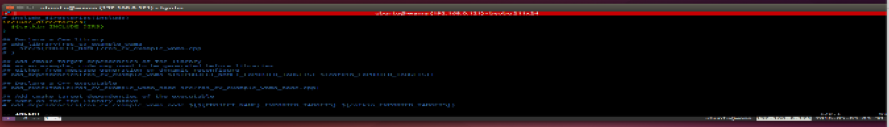
\includegraphics[width=400pt]{pic/5_2_8.png}
    \end{center}
\end{figure}
\begin{figure}[htp]
    \begin{center}
        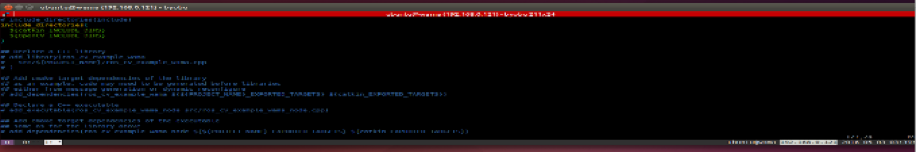
\includegraphics[width=400pt]{pic/5_2_9.png}
    \end{center}
\end{figure}
\\
\\\\\\\\\\\\duckiebot \$ cd src
\\duckiebot \$ cp ~/duckietown/catkin\_ws/src/spring2016\_nctu/wama/ros\_cv\_example\_wama/src/ros\_cv\_example\_wama\_node.py ros\_cv\_example\_duckiebot\_node.py 
\\(指令解釋:將範例python程式複製此目錄底下)
\\\\步驟四、 在此目錄” ros\_cv\_example”創造一個名為launch的資料夾
\\我們會像步驟二一樣去建立launch這個資料夾,之後把之前已經寫好的launch檔複製到此資料夾底下,再進行基本的修改。
\\duckiebot \$ cd ~/duckietown/catkin\_ws/src/summerschool2017\_nctu/duckiebot/ros\_cv\_example
\\duckiebot \$ mkdir launch
\\duckiebot \$ cd launch
\\duckiebot \$ cp ~/duckietown/catkin\_ws/src/spring2016\_nctu/wama/ros\_cv\_example\_wama/launch/ros\_cv\_example\_wama\_node.launch ros\_cv\_example\_duckiebot\_node.launch
\\duckiebot \$ vim ros\_cv\_example\_duckiebot\_node.launch
\\Modify the following: duckiebot=your duckiebot name
\\       <arg name="pkg\_name" default="ros\_cv\_example\_duckiebot" doc="name of the package"/>
\\       <arg name="node\_name" default="ros\_cv\_example\_duckiebot\_node" doc="name of the node"/>
\\(指令解釋:複製範例node檔到這個資料夾,並進行以上修改,目的是因為每個人的鴨子車名都不一樣,因此需要修改。)
\\\\步驟五、使用 catkin\_make 來編譯剛剛建立的package還有寫好的程式
\\在ROS中,當我們創建好package與寫完程式後,為了編譯他們,我們使用catkin\_make(可以看成是cmake的進階版),如果catkin\_make都順利過了,代表程式正確、資料庫鏈結成功,就可以去放心執行了。
\\duckiebot \$ cd ~/duckietown/catkin\_ws
\\(指令解釋:只有進入這個目錄才能進行catkin\_make)
\\duckiebot \$ catkin\_make
\\(指令解釋:進行catkin\_make編譯所有的在此目錄底下的程式)
\\\\步驟六、用launch檔執行package裡的程式
\\在此步驟中,我們要來執行剛剛寫好的程式與launch檔。我們會先在鴨子車執行launch檔,之後在筆電上使用ROS的圖形化模擬環境RVIZ來把傳送的訊息視覺化。
\\duckiebot \$ roslaunch duckietown\_duckiebot ros\_cv\_example\_tim.launch veh:=[duckiebot]
\\(指令解釋:執行launch檔)
\\(附註:以下步驟在筆電上執行)
\\laptop \$ cd ~/duckietown
\\laptop \$ source environment.sh
\\(指令解釋:執行bash檔”environment.sh”)
\\laptop \$ source set\_ros\_master.sh duckiebot
\\(指令解釋:執行bash檔” set\_ros\_master.sh”)
\\laptop \$ rviz 
(指令解釋:開啟圖形化模擬環境rviz)
\\\\RVIZ操作解釋、
\\在RVIZ中請按add鍵加入topic” /duckiebot/ros\_cv\_example\_duckiebot\_node/image\_ros\_cv”,加入後便可以看到圖片。
\subsection{牛刀小試:}
相信經由這一節的解釋,你已了解如何實作ROS package,因此希望你可以使用在本節已創好的ROS package,然後修改執行的python檔”ros\_cv\_example\_duckiebot\_node.py”讓你的程式辨識人臉並顯示在RVIZ上。
\\\\提示、
\\藉由以下指令你可以加入一些 OpenCV 的函式:
\\duckiebot \$ vim ~/duckietown/catkin\_ws/src/summerschool2017\_nctu/duckiebot/ros\_cv\_example\_duckiebot/src\\/ros\_cv\_example\_duckiebot\_node.py
\begin{figure}[htp]
    \begin{center}
        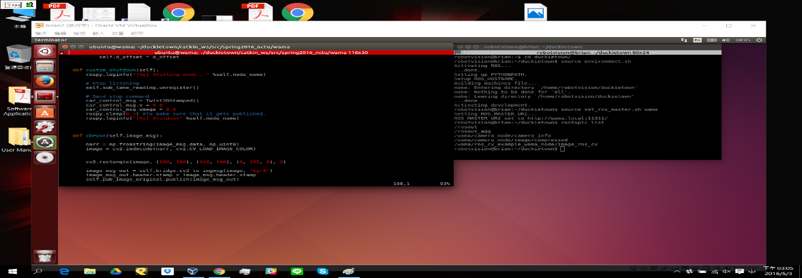
\includegraphics[width=400pt]{pic/5_2_10.png}
    \end{center}
\end{figure}
\\
例如 cv2.rectangle可以幫你的圖形畫一個矩形

\newpage
\section{1-2-3木頭人}
在學習玩前兩節的OpenCV物體辨識演算法與完整建立一個ROS package並且編譯執行後,接著我們要來實作一個專題:1-2-3木頭人,此專題會運用前兩節所學,並且延伸,目標最終是使用搖桿來操作duckiebot,並且如果它有看到人臉它會自動停止。
\\\\先備知識與工具:
\\臉部偵測器 (jupyter-notebook)
\\原本就有的duckietown package
\\	duckietown camera.launch
\\	duckietown joystick.launch
\\你自己的ROS package
\\如何去建立Ros package 
\\	face\_detector\_duckiebot.launch
\\如何去建立 ros launch
\\	onetwothree\_stop\_duckiebot.launch
\subsection{題目介紹:}
架構
\\在此專題中輸入為相機拍攝的影像與搖桿控制,演算法的部分是臉部偵測會持續地進行,如果臉部沒有被偵測到,搖桿控制訊號將會轉成車子馬達的訊號給車子馬達,車子便會移動,但若是有偵測到臉,演算法將會傳送一個停止的訊號給車子馬達,車子便會停下來。
\begin{figure}[htp]
    \begin{center}
        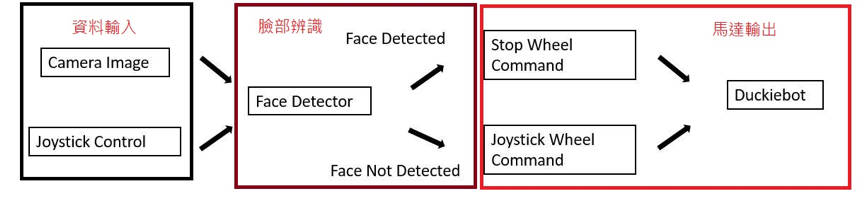
\includegraphics[width=400pt]{pic/5_3_1.png}
    \end{center}
\end{figure}
\\
\subsection{實驗步驟:}
在本次專題練習裡,大部分的程式皆已寫好,但有些讓學生能進行填空已做為對ROS package、ROS node、ROS launch的概念練習,在此四大步驟裡,我們會反覆訓練到如何創建ROS package、如何連結資料庫,如何將ROS node與launch修改完整,最後使用一個launch去呼叫諸多ROS package的launch與node完成1-2-3木頭人的任務。
\\\\步驟一、建立一個launch檔 face\_detector\_duckiebot\_node.launch
\\duckiebot \$ cd ~/duckietown
\\duckiebot \$ source environment.sh
\\(指令解釋:執行bash檔”environment.sh”)
\\duckiebot \$ source set\_ros\_master.sh [duckiebot]
\\(指令解釋:執行bash檔”set\_ros\_master.sh”)
\\duckiebot \$ cd ~/duckietown/catkin\_ws/src/summer\_school/duckiebot
\\\\步驟二、建立一個 ros package
\\duckiebot \$ catkin\_create\_pkg face\_detector\_duckiebot duckietown\_msgs sensor\_msgs rospy cv\_bridge
\\(指令解釋:創造ROS package“face\_detector\_duckiebot”,且加入一些需要用到的函式庫。)
\\duckiebot \$ cd ~/duckietown/catkin\_ws/src/summer\_school/duckiebot /face\_detector\_ duckiebot
\\duckiebot \$  vim CMakeLists.txt 
\\(指令解釋:修改” CMakeLists.txt”,增加“\${OpenCV\_INCLUDE\_DIRS}”與roscpp如下圖)
\begin{figure}[htp]
    \begin{center}
        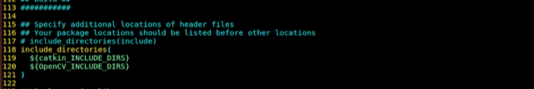
\includegraphics[width=400pt]{pic/5_3_2.png}
    \end{center}
\end{figure}
\\
前:
\begin{figure}[htp]
    \begin{center}
        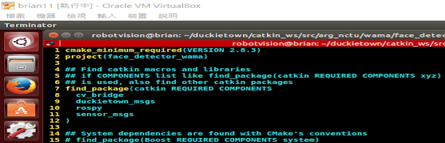
\includegraphics[width=300pt]{pic/5_3_3.png}
    \end{center}
\end{figure}
\\
後:
\begin{figure}[htp]
    \begin{center}
        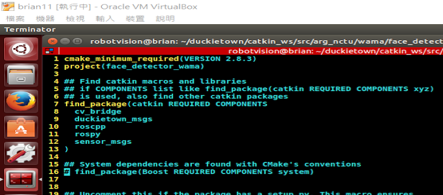
\includegraphics[width=300pt]{pic/5_3_4.png}
    \end{center}
\end{figure}
\\
\\duckiebot \$ cd ~/duckietown/catkin\_ws/src/summer\_school/duckiebot/face\_detector\_duckiebot
\\duckiebot \$  vim package.xml
(指令解釋:修改” package.xml”,增加“roscpp”如下圖)
\begin{figure}[htp]
    \begin{center}
        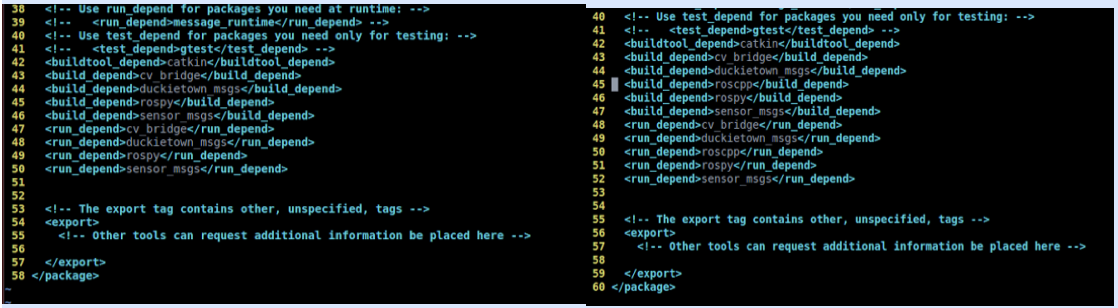
\includegraphics[width=400pt]{pic/5_3_5.png}
    \end{center}
\end{figure}
\\
\\duckiebot \$ cd ~/duckietown/catkin\_ws/src/summer\_school/duckiebot /face\_detector\_ duckiebot
\\duckiebot \$ mkdir launch
\\duckiebot \$ cd ~/duckietown/catkin\_ws/src/summer\_school/duckiebot/face\_detector\_duckiebot/launch
\\duckiebot \$ cp ~/duckietown/tutorials/ros/face\_detector\_tutorial\_node.launch face\_detector\_detector\_node.launch
\\duckiebot \$ vim face\_detector\_tutorial\_node.launch
\\(指令解釋:開啟” face\_detector\_tutorial\_node.launch”,並將程式裡所有XXX修改成你的鴨子車名)
\begin{figure}[htp]
    \begin{center}
        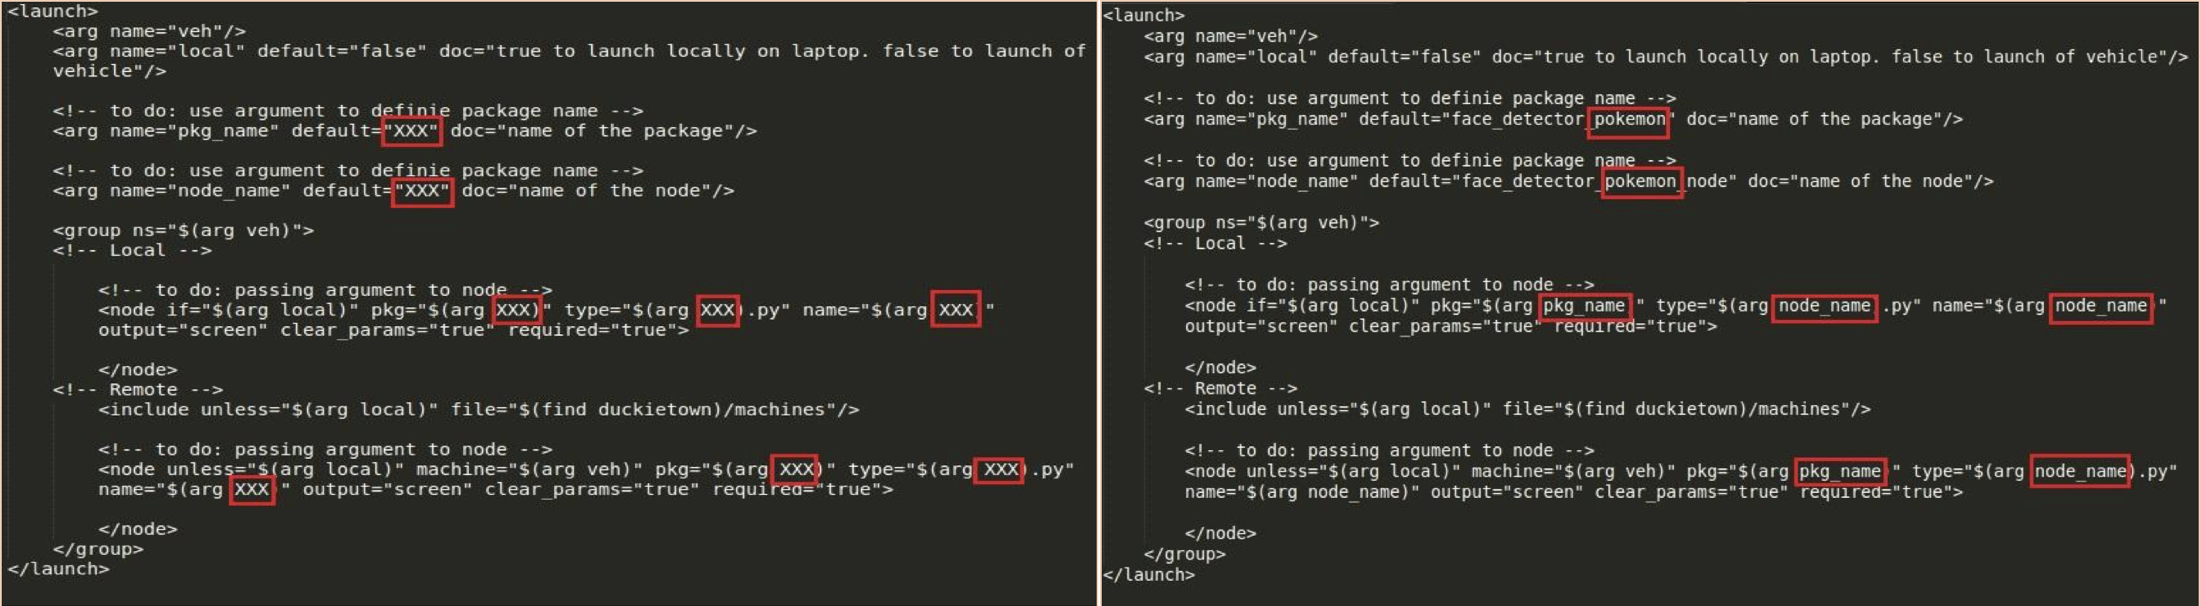
\includegraphics[width=400pt]{pic/5_3_10.png}
    \end{center}
\end{figure}
\\
步驟三、建立一個python檔 face\_detector\_duckiebot\_node.py
\\duckiebot \$ cd ~/duckietown/catkin\_ws/src/summer\_school/duckiebot/face\_detector\_duckiebot
\\(指令解釋:進入資料夾” face\_detector\_duckiebot”)
\\duckiebot \$ mkdir src
\\(指令解釋:創建新資料夾”src”)
\\duckiebot \$ cp ~/duckietown/tutorials/ros/face\_detector\_tutorial\_node.py face\_detector\_duckiebot\_node.py
\\(指令解釋:複製” face\_detector\_tutorial\_node.py”到此資料夾底下)
\\duckiebot \$ vim face\_detector\_duckiebot\_node.py
\\(指令解釋:開啟face\_detector\_duckiebot\_node.py,並改成如下圖所示)
\begin{figure}[htp]
    \begin{center}
        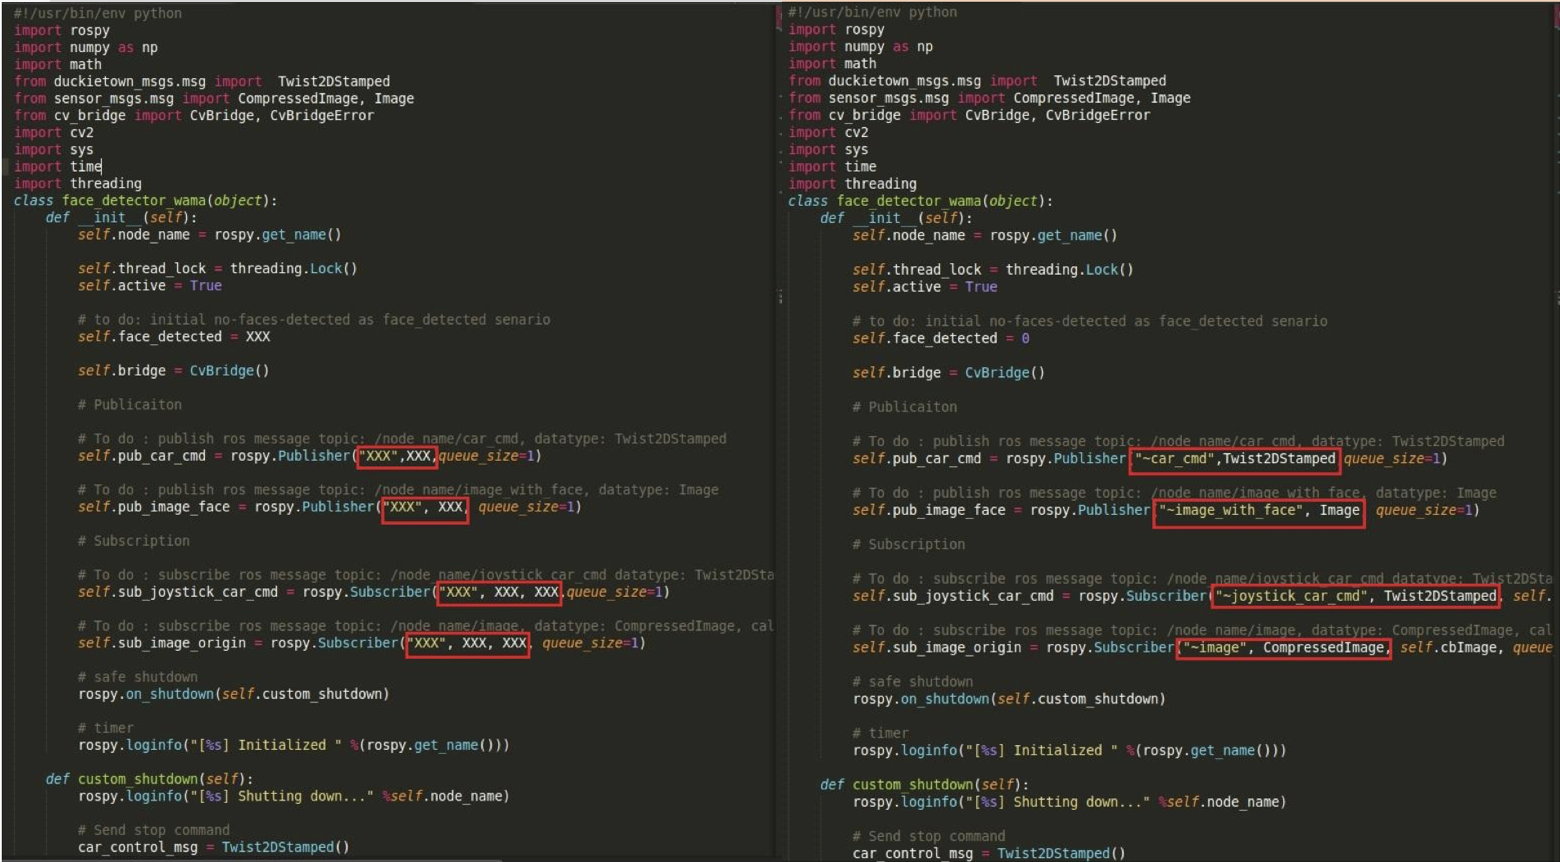
\includegraphics[width=400pt]{pic/5_3_11.png}
    \end{center}
\end{figure}
\\\\\\\\\\\\\\\\\\
\\duckiebot \$ cd ~/duckietown/catkin\_ws
\\duckiebot \$ catkin\_make
\\(指令解釋:進行catkin\_make編譯所有的在此目錄底下的程式)
\\duckiebot \$ roslaunch face\_detector\_duckiebot face\_detector\_duckiebot\_node.launch veh:= duckiebot
\\(指令解釋:執行launch檔確定以上操作是否成功)
\\\\步驟四、創建還有測試 onetwothree\_stop\_duckiebot.launch	
\\duckiebot \$ cd ~/duckietown/catkin\_ws/src/fall2016\_nctu/duckiebot
\\duckiebot \$ catkin\_create\_pkg duckietown\_nctu\_duckiebot
\\(指令解釋:創造ROS package “duckietown\_nctu\_duckiebot”)
\\duckiebot \$ cd ~/duckietown/catkin\_ws/src/fall2016\_nctu/duckiebot /duckietown\_nctu\_duckiebot
\\duckiebot \$ mkdir launch
\\(指令解釋:創建資料夾”launch”)
\\duckiebot \$ cd ~/duckietown/catkin\_ws/src/fall2016\_nctu/duckiebot /duckietown\_nctu\_duckiebot/launch
\\duckiebot \$ cp ~/duckietown/tutorials/ros/onetwothree\_stop\_tutorial.launch onetwothree\_stop\_duckiebot.launch
\\(指令解釋:複製” onetwothree\_stop\_tutorial.launch”到此資料夾裡)
\\duckiebot \$ cd ~/duckietown/catkin\_ws
\\duckiebot \$ catkin\_make
\\(指令解釋:進行catkin\_make編譯所有的在此目錄底下的程式)
\\duckiebot \$ roslaunch duckietown\_nctu\_duckiebot onetwothree\_stop\_duckiebot.launch veh:=duckiebot
\\(指令解釋:執行launch檔” onetwothree\_stop\_duckiebot.launch”)


\end{document}

















